% no answer key
\documentclass[letterpaper, landscape]{exam}
\usepackage{2in1, lscape} 

% answer key
\printanswers{}

\usepackage{units} 
\usepackage{graphicx}
\usepackage[fleqn]{amsmath}
\usepackage{cancel}
\usepackage{float}
\usepackage{mdwlist}
\usepackage{booktabs}
\usepackage{polynom}
\usepackage{caption}
\usepackage{fullpage}
\usepackage{comment}
\usepackage{enumerate}
\usepackage{parskip}
\usepackage{xfrac}

\newcommand{\degree}{\ensuremath{^\circ}} 
\everymath{\displaystyle}

% \printanswers
\excludecomment{comment}
\addpoints{}

\title{Statistics \\ Part One Exam}
\date{\today}
\author{}

\begin{document}

  \maketitle

  % \begin{center}
  %   \gradetable[h][pages]
  % \end{center}

  \section{Instructions}
  Show all your work and explain your answers---a correct guess won't receive credit without
  work/explanation. 
  
  An incorrect answer will receive partial credit if you understand the
  concept but made an arithmetic mistake.

  \section{Questions}

  \begin{questions}

    \question[5] Ten people in a room have an average height of 5 feet 6 inches.
    An eleventh person who is 6 feet 5 inches tall enters the room. What is the
    mean height of all 11 people? 

    \begin{solution}
      It's easiest to do this problem in inches.

      The people already in the room are 66 inches tall. The new arrival is 77
      inches tall. The new mean is:
      \[
        \bar{x} = \frac{10 \cdot 66 + 77}{11} = \unit[67]{in}
      \]

      You can convert back to feet if you want: 67 inches is 6 feet 5 inches
    \end{solution}

    \question[5] Average hourly earnings are computed each month by the Bureau
    of Labor Statistics as the total wages paid divided by the total hours
    worked. During recessions, average hourly earnings typically go up. When the
    recession ends, average hourly earnings often decline.  Explain how this can
    happen, even if nobody gets a raise or a pay cut. 

    \begin{solution}
      In a recession the lower-paid inexperienced people are the first ones to
      get laid off, leaving only the higher paid, more experienced people. The
      average pay goes up since you're only averaging the higher-paid people's
      wages.
    \end{solution}

    \question[5] For US citizens age 25 and over, which would be higher: mean or
    median income?  Explain.

    \begin{solution}
      Income is right-skewed. Most people are clustered toward the bottom, but
      there are a few people like Bill Gates and Jeff Bezos who make billions of
      dollars.

      The mean is affected by the small number of high-earners, so it will be
      higher than the median.
    \end{solution}

    \question{}\label{q:chol}
      \begin{table}[ht]
        \centering
        \begin{tabular}{rlrl}
          \toprule
          Cholesterol & Sex & Cholesterol & Sex \\
          \midrule
          690         & M   & 98          & F \\
          466         & M   & 94          & F \\
          649         & M   & 318         & F \\
          172         & M   & 280         & F \\
          265         & M   & 223         & F \\
          176         & M   & 596         & F \\
          957         & M   & 62          & F \\
          121         & M   & 149         & F \\
          613         & M   & 2           & F \\
           31         & M   & 309         & F \\
          \bottomrule
        \end{tabular}
        \caption{Question~\ref{q:chol}}\label{tab:chol}
      \end{table}

      Table~\ref{tab:chol} shows cholesterol data for a sample of men and women.

      \begin{parts}
        \part[10] 
          Draw a histogram with bin width 100 for the cholesterol data in
          Table~\ref{tab:chol}, including both men and women combined.

          \ifprintanswers{}
            \begin{figure}[H]
              \centering
              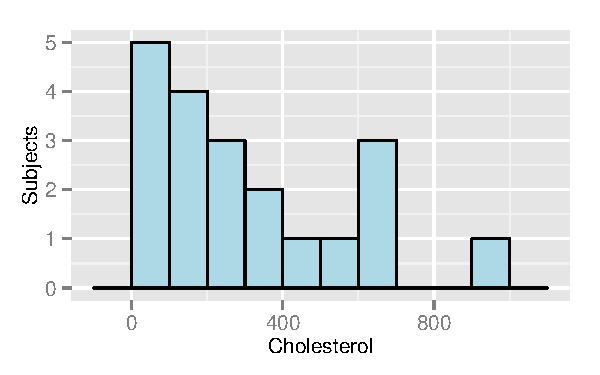
\includegraphics{figures/cholesterol_histogram.pdf}
              \caption{Cholesterol}\label{fig:chol}
            \end{figure}
          \fi

        \part[3] Without calculating the mean or median, is the mean value
        higher or lower than the median? Explain how you know.

        \part[7] Calculate the 5-number summary for the men.

        \ifprintanswers{}
          \begin{table}[ht]
            \centering
            \begin{tabular}{lr}
              \toprule
              Min & 31 \\
              Q1  & 172 \\
              Med & 365.5 \\
              Q3  & 649 \\
              Max & 957 \\
              \bottomrule
            \end{tabular}
          \end{table}
        \fi
        
        \part[7] Calculate the 5-number summary for the women.

        \ifprintanswers{}
          \begin{table}[ht]
            \centering
            \begin{tabular}{lr}
              \toprule
              Min & 2 \\
              Q1  & 94 \\
              Med & 186 \\
              Q3  & 309 \\
              Max & 596 \\
              \bottomrule
            \end{tabular}
          \end{table}
        \fi

        \part[8] Draw a box plot comparing the men to the women.

          \ifprintanswers{}
            \begin{figure}[H]
              \centering
              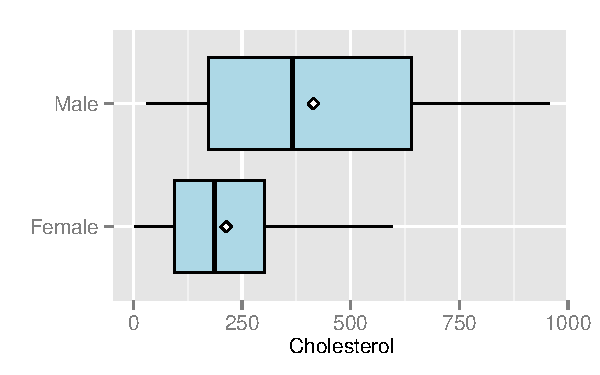
\includegraphics{figures/cholesterol_box.pdf}
              \caption{Cholesterol}\label{fig:chol}
            \end{figure}
          \fi

        \part[3] 
          Are there any outliers among the men, when compared to other men? 

          \begin{solution}
            Calculate the IQR\@:
            \[
              IQR = 1.5 (649 - 172) = 715.5
            \]

            To qualify as an outlier, somebody would need to have a number higher
            than:
            \[
              649 + 715.5 = 1364.5
            \]

            The maximum value is 957, so nobody is an outlier.
          \end{solution}

      \end{parts}

    \ifprintanswers{}
    \else
      \newpage
    \fi

    \question{}
      Heights have an approximately Normal distribution of $N(69.9, 2.8)$
      inches.

    \begin{parts}
      \part[5] 
        The mean height of an NBA player is 6 ft 7 in. What percentage of
        men are shorter than this?

        \begin{solution}
          \begin{align*}
            z & = \frac{79 - 69.9}{2.8} \\
              & = 3.25 \\
          \end{align*}

          From Table A, \fbox{ 99.94\% } of men are shorter than this.

        \end{solution}

      \part[5] Ski jumpers tend to be shorter than basketball players. The
      z-score for a mean-height ski jumper is: 
      \[
        z = 0.3739
      \]
      
      What is the mean height of ski-jumpers, in inches?

      \begin{solution}
        \begin{align*}
          z & = \frac{x - \mu}{\sigma} \\
          x & = z \sigma + \mu \\
          \\
          x & = 0.3739 \cdot 2.8 + 69.9 \\
            & \approx \boxed{ \unit[70.95]{in} } \\
        \end{align*}
      \end{solution}

    \end{parts}

    \question{}\label{q:sat}

      ACT and SAT test scores follow approximately Normal distributions. See
      Table~\ref{tab:sat} for the mean and standard deviation.

      \begin{table}[H]
        \centering
        \begin{tabular}{lrr}
          \toprule
              & $\mu$ & $\sigma$ \\
          \midrule
          SAT & 1518  & 325 \\
          ACT & 21.1  & 4.8 \\
          \bottomrule
        \end{tabular}
        \caption{Question~\ref{q:sat}}\label{tab:sat}
      \end{table}

      \begin{parts}
        \part[5] Which is a better score?
          \begin{itemize*}
            \item a score of 1150 on the SAT
            \item a score of 16.5 on the ACT
          \end{itemize*}

          \begin{solution}
            The best score will be the one that with the largest z-score.

            \begin{align*}
              z_{sat} & = \frac{1150 - 1518}{325} \\
                      & = -1.1323 \\
              \\
              z_{act} & = \frac{16.5 - 21.1}{4.8} \\
                      & = -0.9583 \\
            \end{align*}

            Both scores are bad, but the ACT score is less bad.

          \end{solution}

        \part[5] the University of Southern North Dakota at Hoople requires a
          score in the 95th percentile in both tests. What scores do you need to get,
          in order to get in to USNDH\@?

          \begin{solution}
            The 95th percentile corresponds to a z-score of 1.6449.

            \begin{align*}
              \text{SAT} & = 1.6449 \cdot 325 + 1518 \approx \boxed{ 2053 } \\
              \text{ACT} & = 1.6449 \cdot 4.8 + 21.1 \approx \boxed{ 29 } \\
            \end{align*}
          \end{solution}

      \end{parts}

      \question{}\label{q:cancer}

      Some counties in Oregon have been exposed to high radiation levels because
      of the nuclear research at Hanford.  Table~\ref{tab:cancer} shows the
      radiation exposure and cancer mortality rates for some of these counties.

      The correlation coefficient for Exposure/Mortality is: $r = 0.9263$

      \begin{table}[ht]
        \centering
        \begin{tabular}{lrr}
          \toprule
                    & $\bar{x}$ & $s$    \\
          \midrule              
          Exposure  & 4.6178    & 3.4911 \\
          Mortality & 157.34    & 34.79  \\
          \bottomrule
        \end{tabular}
      \end{table}

      \begin{table}[ht]
        \centering
        \begin{tabular}{lrr}
          \toprule
          County     & Exposure & Mortality \\
          \midrule
          Umatilla   & 2.49     & 147.10 \\
          Morrow     & 2.57     & 130.10 \\
          Gilliam    & 3.41     & 129.90 \\
          Sherman    & 1.25     & 113.50 \\
          Wasco      & 1.62     & 137.50 \\
          Hood River & 3.83     & 162.30 \\
          Portland   & 11.64    & 207.50 \\
          Columbia   & 6.41     & 177.90 \\
          Clatsop    & 8.34     & 210.30 \\
          \bottomrule
        \end{tabular}
        \caption{Question~\ref{q:cancer} (from study by Fadely)}\label{tab:cancer}
      \end{table}


      \begin{parts}
        \part[6] Draw a scatter plot for this data, using the exposure rate as
        the explanatory variable.

          \ifprintanswers{}
            \begin{figure}[H]
              \centering
              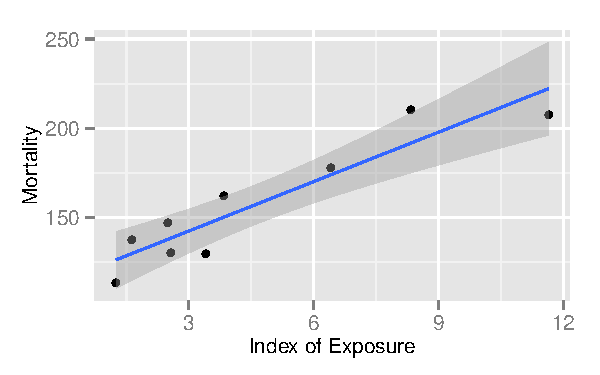
\includegraphics{figures/cancer.pdf}
              \caption{Cholesterol}\label{fig:chol}
            \end{figure}
          \fi

        \part[7] Find the equation of the linear regression line for mortality
        with exposure as the explanatory variable.

          \begin{solution}
            \[
              y = 9.231 \cdot x + 114.72
            \]
          \end{solution}

        \part[2] Draw the regression line on your graph.

          \begin{solution}
            See Figure~\ref{fig:chol}
          \end{solution}

        \part[2] If some other county had an exposure of 5.00, what might you
        expect the mortality to be in that county, based on your regression
        equation?

        \begin{solution}
          \[
            y = 9.231 \cdot 5 + 114.72 \approx 160.88 \\
          \]

        \end{solution}

        \part[3] What percentage of the variation in cancer rate is explained by
        variation in radiation exposure?

        \begin{solution}
          $r^2 = 0.9263^2 \approx 85.80\% $
        \end{solution}

        \part[7] 
        
        If you instead wanted to go the other direction and find probable exposure given mortality
        rate, what is the equation for this regression line?
        % \[
        %   \text{exposure} = 0.1083 \times \text{cancer} - 12.46
        % \]

        \begin{solution}
          \[
            y = 0.09296 x - 10.01
          \]
        \end{solution}

      \end{parts}
  \end{questions}

\end{document}

